\section{Navigierbarkeit}
\label{sec:Kap-8.4}

Die UML bietet die Möglichkeit, (Klassen)Assoziationen und (Objekt)Verbindungen mit Navigierbarkeiten zu versehen. Dafür werden die Enden der Linien zwischen den Klassen bzw. Objekten um Pfeilspitzen ergänzt. Die Navigierbarkeit erlaubt es, die Interaktion zwischen den Objekten und die Rollen, die Objekte einnehmen können (Dienstleister und/oder Dienstnutzer) genauer zu spezifizieren. Die UML unterscheidet zwischen
\begin{itemize}
	\item \textit{navigierbar}, mit den Formen
	\begin{itemize}
		\item \textit{unidirektional navigierbar} und 
		\item \textit{bidirektional navigierbar}, 
	\end{itemize}
	\item \textit{nicht navigierbar} und
	\item \textit{unspezifiziert}.
\end{itemize}

Die Navigierbarkeit einer Beziehung sagt aus, inwiefern sich die verbundenen Elemente kennen oder nicht kennen, also je nach Metapher: sich Nachrichten schicken können, als Dienstleister auftreten können, Operationen des anderen aufrufen können. Wenn ein Objekt ein anderes Objekt kennt, kann es dessen Dienstleistungen nutzen, indem es Operationen des anderen Objekts aufruft. Auf einer implemen\-tierungs\-technischen Ebene bedeutet Navigierbarkeit, dass ein Objekt einer Klasse~A, die Klasse~B kennt, ein Attribut vom Datentyp der Klasse B besitzt. 

Die Verbindungen und Assoziationen in den Abbildungen in Kapitel~4
(durchgezogene Linien ohne Pfeilspitzen) waren bezüglich der Navigierbarkeit alle unspezifiziert. Unspezifiziert bedeutet, dass wir uns zum Erstellungszeitpunkt des Klassen\-diagramms noch keine Gedanken darüber gemacht haben, ob zum Beispiel (Abb.~4.12 in Kap.~4) % TODO (Abb.~\ref{fig:klassendiagramm_zu_objektdiagramm} in Kap.~\ref{sed:Kap-3}) 
eine Lehrer-Instanz Operationen einer Fach-Instanz aufrufen können soll und/oder umgekehrt. In Domänenklassendiagrammen findet man häufig noch unspezifizierte Navigierbarkeiten. Im Laufe von Entwurfsaktivitäten oder spätestens während der Implementierung müssen Navigierbarkeitsentscheidungen getroffen werden. 

\vspace{\baselineskip} %%% für Druck

\begin{figure}[h!]
	\centering
	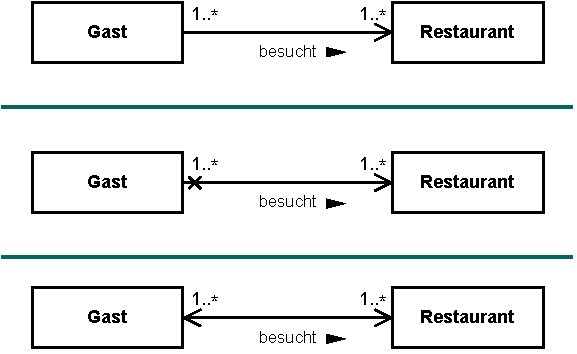
\includegraphics[scale=1.0]{Bilder/Kapitel-8/navigierbarkeiten_gast_restaurant.pdf}
	\caption{Navigierbarkeiten}
	\label{fig:navigierbarkeiten_gast_restaurant}
\end{figure}

\pagebreak %%% für Druck

Abbildung~\ref{fig:navigierbarkeiten_gast_restaurant} zeigt weitere Formen der Navigierbarkeit in UML. Bei der unidirektionalen Navigierbarkeit kennt eine Klasse die andere, aber nicht umgekehrt. Dies wird durch einen Pfeil am Assoziationsende der Dienstleister-Klasse modelliert. In unserem Beispiel ganz oben kennt die Klasse \sttpUMLText{Gast} die Klasse \sttpUMLText{Restaurant}. Eine Gast-Instanz kann somit Operationen einer Restaurant-Instanz aufrufen, umgekehrt jedoch nicht. Eine saubere Modellierung unidirektionaler Navigierbarkeit erfordert seit UML~2 die Kennzeichnung desjenigen Assoziationsendes mit einem {\Large$\times$}, in dessen Richtung nicht navigiert werden darf (Abb.~\ref{fig:navigierbarkeiten_gast_restaurant} Mitte): Das {\Large$\times$} bedeutet nicht navigierbar. Die obere Abbildung in Abbildung~\ref{fig:navigierbarkeiten_gast_restaurant} stellt daher streng genommen keine unidirektionale Navigierbarkeit dar, sondern eine nur teilweise spezifizierte Navigierbar\-keit. Hier hat sich die Bedeutung zwischen UML~1 und UML~2 verändert. In der Praxis wird man aber auch bei Verwendung von UML~2 häufig auf Darstellungen wie Abbildung~\ref{fig:navigierbarkeiten_gast_restaurant} oben treffen, mit denen unidirektionale Navigierbarkeit ausgedrückt werden soll. Solange alle Beteiligten eines Softwareentwicklungsprojekts den verwendeten Modellierungselementen dieselbe Bedeutung zuweisen, ist das auch unproblematisch.

Abbildung~\ref{fig:navigierbarkeiten_gast_restaurant} unten zeigt die UML-Darstellung für bidirektionale Navigierbarkeit. Die Klassen \sttpUMLText{Gast} und \sttpUMLText{Restaurant} kennen sich gegenseitig. Somit können sowohl Instanzen der Klasse \sttpUMLText{Gast} als auch Instanzen der Klasse \sttpUMLText{Restaurant} in den beiden Rollen Dienstleister und Dienstnutzer auftreten. Aufgrund diesbezüglicher Änderungen zwischen UML~1 und UML~2 werden auch unspezifizierte Navigierbarkeiten (ohne Pfeilspitzen) in der Praxis häufig als bidirektional interpretiert. Die saubere Variante Bidirektionalität in UML~2 zu modellieren ist aber, sie auch explizit mit Pfeilspitzen an beiden Assoziationsenden auszudrücken.

\begin{figure}[h!]
	\centering
	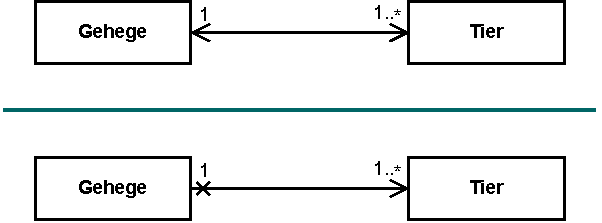
\includegraphics[scale=1.0]{Bilder/Kapitel-8/navigierbarkeit_tier.pdf}
	\caption{Navigierbarkeit in der Beziehung zwischen \sttpUMLText{Tier} und \sttpUMLText{Gehege}}
	\label{fig:navigierbarkeit_tier}
\end{figure}

Ein Beispiel aus dem Zookontext: Abbildung~\ref{fig:navigierbarkeit_tier} zeigt zwei Möglichkeiten, wie \mbox{eine} inhaltlich sinnvolle Beziehung zwischen den Klassen \sttpUMLText{Tier} und \sttpUMLText{Gehege} aussehen könnte. Im oberen Fall kennt die Klasse \sttpUMLText{Tier} die Klasse \sttpUMLText{Gehege}, im unteren Fall nicht. Die Klasse \sttpUMLText{Gehege} wiederum kennt in beiden Fällen die Klasse \sttpUMLText{Tier}. In dieser Richtung keine Navigierbarkeit vorzusehen, wäre nicht sinnvoll. Denn dann müsste man jedes Mal, wenn man wissen möchte, welche Tiere sich in einem bestimmten \mbox{Gehege} befinden, alle Tier-Objekte durchsuchen und prüfen, ob sie mit dem gesuchten Gehege-Objekt verbunden sind und wenn ja, sie sich in einer zusätzlichen Datenstruktur „merken“. Nach der Beschreibung des Tiererfassungsprozesses (S.~\pageref{sec:Kap-8.2:Tiererfassung}) würde der untere Fall von Abbildung~\ref{fig:navigierbarkeit_tier} ausreichen. Wenn aber bei den Informa\-tionen auf der Tier-Detailseite des Tierinformationssystems nachher auch das \mbox{Gehege} aufgeführt sein soll, in dem das Tier aktuell lebt und das Tier vielleicht im Laufe seines Lebens das Gehege sogar wechselt, ist eine bidirektionale Navi\-gierbar\-keit wie im oberen Fall von Abbildung~\ref{fig:navigierbarkeit_tier} sinnvoller. 

\begin{figure}[h!]
	\centering
	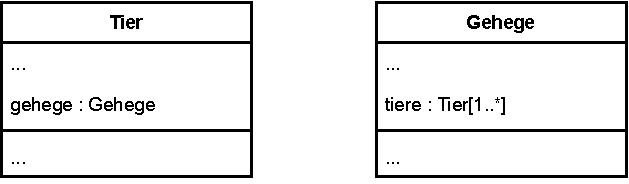
\includegraphics[scale=1.0]{Bilder/Kapitel-8/klassen_tier_und_gehege.pdf}
	\caption{Die Klassen \sttpUMLText{Tier} und \sttpUMLText{Gehege}}
	\label{fig:klassen_tier_und_gehege}
\end{figure}

Wie Sie an diesem -- zugegebenermaßen stark konstruierten -- Beispiel sehen, ist die Festlegung der Navigierbarkeiten zwischen Klassen kompliziert. Man muss insbesondere das vorgesehene Nutzungsverhalten der verschiedenen Akteure mit dem Softwaresystem berücksichtigen. Vorsichtshalber überall bidirektionale Navigierbarkeit vorzusehen, ist aber auch nicht sinnvoll. Abbildung~\ref{fig:klassen_tier_und_gehege} zeigt, wie sich in unserem Beispiel die bidirektionale Navigierbarkeit zwischen den beiden Klassen später als Attribute der Klassen im Programmcode darstellen würde. Man benötigt für Fälle, in denen beide Klassen jeweils ein Attribut mit Datentyp der anderen Klasse haben, immer einen Mechanismus, der sicherstellt, dass bei Änderungen die entsprechenden Objekte beider Klassen konsistent gehalten werden. Diesen Aufwand kann man sich bei unidirektionaler Navigierbarkeit ersparen.

Zum 
\marginline{Navigierbarkeit vs. Multiplizitäten}
Abschluss des Themas Navigierbarkeit möchten wir noch auf den wichtigen Unterschied zwischen a) dem \textbf{Vorhandensein} einer Beziehung und b) der \textbf{Navi\-gierbar\-keit} dieser Beziehung hinweisen. Betrachten Sie das Klassendiagramm in Abbildung~\ref{fig:multiplizitaeten_und_navigierbarkeit} oben und die drei mit den Nummern 1 bis 3 gekennzeichneten Objekt\-konstella\-tionen in derselben Abbildung unten. Handelt es sich um gültige oder ungültige Objektkonstellationen?

\begin{figure}[h!]
	\centering
	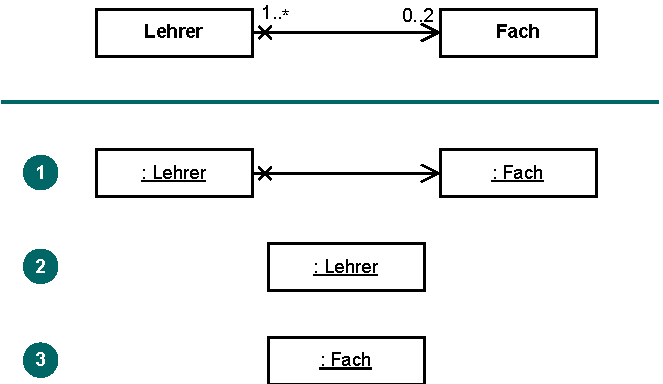
\includegraphics[scale=1.0]{Bilder/Kapitel-8/multiplizitaeten_und_navigierbarkeit.pdf}
	\caption{Multiplizitäten und Navigierbarkeit.}
	\label{fig:multiplizitaeten_und_navigierbarkeit}
\end{figure}

Objektkonstellation Nr.~1 ist einfach zu entscheiden: Sie ist gültig, da es zu einer Lehrer-Instanz maximal zwei verbundene Fach-Instanzen geben darf und zu einer Fach-Instanz mindestens eine verbundene Lehrer-Instanz geben muss. Außerdem muss die Verbindung uni\-di\-rek\-tio\-nal navigierbar von Lehrer-Instanz zu Fach-Instanz sein. Die dargestellte uni\-di\-rek\-tio\-na\-le 1-zu-1-Beziehung zwischen einer Lehrer- und einer Fach-Instanz erfüllt diese Regeln. Objektkonstellation Nr.~2 ist ebenfalls gültig, da es aufgrund der \sttpUMLText{0..2} Multiplizität auch Lehrer-Instanzen geben kann, die keine Verbindung zu einer Fach-Instanz haben. Objektkonstellation Nr.~3 ist ungültig. Wenn Sie jetzt irritiert sind, ist Ihnen das passiert, was UML-Anfängern häufig passiert: Man konzentriert sich auf die Navigierbarkeit der Beziehung und missachtet die Multiplizitäten. Die Navigierbarkeit von Fach-Instanz zu Lehrer-Instanz ist ausdrücklich ausgeschlossen, doch die Multiplizität \sttpUMLText{1..*} sagt aus, dass es zu jeder Fach-Instanz mindestens eine Lehrer-Instanz geben muss. Eine unverbun\-dene Fach-Instanz wie in Objektkonstellation Nr.~3 darf es daher nicht geben. Diese Fach-Instanz kann zwar niemals auf die Operationen einer mit ihr verbundenen Lehrer-Instanz zugreifen, nichtsdestotrotz muss es die Verbindung zwischen diesen Instanzen geben. Implementierungstechnisch muss die durch das Klassendiagramm vorgegebene Lehrer-Fach-Beziehung so gelöst werden, dass immer wenn ein Objekt vom Typ \sttpUMLText{Fach} erzeugt wird, gleichzeitig auch mindestens ein Objekt vom Typ \sttpUMLText{Lehrer} erzeugt wird, sofern es die für die Verbindung benötigte Lehrer-Instanz noch nicht gibt. Zusätzlich muss von der neu erzeugten oder schon vorhandenen Lehrer-Instanz eine Referenz auf die neu erzeugte Fach-Instanz gesetzt werden. Die Erzeugung neuer Objekte zur Laufzeit bildet also stets eine Einheit mit der Erzeugung und/oder Verknüpfung weiterer, entsprechend der Regeln des Klassendiagramms notwendiger, Objekte. Dieses Erzeugen und Verknüpfen weiterer Objekte wiederum kann eine Kaskade zusätzlicher Objekt-Erzeugungen und -Verknüpfungen auslösen.